\documentclass[10pt,twocolumn,letterpaper]{article}

% Barang saya sendiri
\usepackage{booktabs}
% \usepackage{caption}
% \captionsetup[table]{skip=8pt}   % Hanya memberi kesan kepada jadual
\usepackage{stfloats}  % Tambahkan ini pada preamble
\usepackage{float}
\usepackage[T1]{fontenc}

\usepackage{cvpr}
\usepackage{times}
\usepackage{epsfig}
\usepackage{graphicx}
\usepackage{amsmath}
\usepackage{amssymb}


\usepackage[breaklinks=true,bookmarks=false]{hyperref}
\cvprfinalcopy % *** Nyahulangkan baris ini untuk penyerahan akhir

\makeatletter
\def\abstract{%
  \centerline{\large\bf Abstrak}% <-- your new label
  \vspace*{12pt}%
  \it%
}
\makeatother

\renewcommand{\tablename}{Jadual}  % now \caption will say “Tabla 1” instead of “Table 1”
\renewcommand{\figurename}{Rajah}   % or whatever you like instead of "Hình"

\def\cvprPaperID{****} % *** Masukkan ID Kertas CVPR di sini
\def\httilde{\mbox{\tt\raisebox{-.5ex}{\symbol{126}}}}

% Halaman bernombor dalam mod penyerahan, dan tidak bernombor dalam versi kamera-siap
%\ifcvprfinal\pagestyle{empty}\fi
\setcounter{page}{1}
\begin{document}

%%%%%%%%% TAJUK
\title{Pengenalan Berdasarkan Data ECDO Bahagian 1/2: Kefahaman Semasa Teori “Earth Flip” Ayunan Dzhanibekov Pemisahan Teras-Selaput Eksotermik (ECDO)}

\author{Junho\\
Diterbitkan Februari 2025\\
Laman web (Muat turun kertas di sini): \href{https://sovrynn.github.io}{sovrynn.github.io}\\
Repo Penyelidikan ECDO: \href{https://github.com/sovrynn/ecdo}{github.com/sovrynn/ecdo}\\
{\tt\small junhobtc@proton.me}
}
\maketitle
%\thispagestyle{empty}

\begin{abstract}
Pada Mei 2024, seorang penulis dalam talian tanpa nama dengan gelaran “The Ethical Skeptic” \cite{0} telah berkongsi satu teori revolusioner yang dipanggil Exothermic Core-Mantle Decoupling Dzhanibekov Oscillation (ECDO) \cite{1}. Teori ini mencadangkan bahawa Bumi pernah mengalami perubahan mendadak dan bencana pada paksi putarannya, yang menyebabkan banjir besar di seluruh dunia apabila lautan melimpahi benua akibat inersia putaran. Selain itu, teori ini membentangkan proses geofizik dan data yang menerangkan serta menunjukkan bahawa satu lagi kejadian seperti ini mungkin akan berlaku tidak lama lagi. Walaupun ramalan bencana banjir dan hari kiamat seperti ini bukanlah sesuatu yang baharu, teori ECDO mempunyai tarikan yang unik kerana pendekatannya yang saintifik, moden, pelbagai disiplin, dan berasaskan data.

Kertas ini adalah bahagian pertama daripada dua ringkasan padat mengenai enam bulan penyelidikan bebas \cite{2,20} terhadap teori ECDO. Ia menyoroti tiga perkara utama:

\begin{flushleft}
\begin{enumerate}
    \item 'Bumi terbalik' seperti ECDO telah berlaku beberapa kali dalam sejarah manusia baru-baru ini, dibuktikan melalui mitos banjir serta tanda-tanda geologi berlakunya banjir besar di benua.
    \item Arah dan magnitud anggaran 'Bumi terbalik' pada masa lalu boleh ditentukan.
    \item Data geomagnetik dan geofizik terkini menunjukkan bahawa satu lagi peristiwa 'Bumi terbalik' mungkin akan berlaku, dan perubahan iklim mungkin disebabkan oleh perubahan dari dalam Bumi, bukannya manusia.
\end{enumerate}
\end{flushleft}

Selain itu, saya membincangkan fizik penyebab di sebalik “Bumi terbalik” yang dicadangkan oleh teori ECDO.

Dalam kertas ini, saya kekal objektif dengan menumpukan pada data kukuh, mengelak bahagian teori yang menarik tetapi spekulatif, dan menegaskan bahawa ini adalah topik yang sangat perlu dikaji dengan lebih mendalam oleh manusia.
\end{abstract}
\section{Pengenalan}

Kisah tentang banjir besar bukanlah perkara baru - malah, ia terdapat dalam setiap budaya utama di seluruh dunia, merangkumi semua tamadun. Memetakan (Rajah \ref{fig:1}) satu kompilasi 267 kisah banjir \cite{3} menunjukkan bahawa hampir semua kawasan yang didiami di Bumi mengandungi kisah tentang banjir.

\begin{figure}[h]
\begin{center}
% \fbox{\rule{0pt}{2in} \rule{0.9\linewidth}{0pt}}
   \includegraphics[width=1\linewidth]{b.png}
\end{center}
   \caption{Lokasi kisah banjir di seluruh dunia \cite{3}.}
\label{fig:1}
\label{fig:onecol}
\end{figure}

Jika diteliti lebih dekat, kisah-kisah banjir ini menunjukkan bahawa ia bukanlah banjir biasa, sebaliknya, ia adalah malapetaka yang dahsyat disertai banjir yang menyapu bersih benua-benua.

\subsection{Kisah Malapetaka Orang Asli Amerika}

Kisah Orang Asli Amerika mengandungi antara catatan paling jelas tentang malapetaka besar di Bumi. Kaum Hopi, satu suku Orang Asli Amerika yang tinggal di timur laut Arizona, berkata bahawa, \textit{"..Sótuknang memanggil Orang Semut supaya membuka dunia bawah tanah mereka untuk orang yang terpilih. Apabila mereka berada dengan selamat di bawah tanah, Sótuknang memerintahkan si kembar, Pöqánghoya dan Palöngawhoya, supaya meninggalkan tempat mereka di hujung utara dan selatan paksi dunia, di mana mereka ditempatkan untuk memastikan bumi berputar dengan betul. \textbf{Si kembar itu baru sahaja meninggalkan tempat mereka apabila dunia, tanpa sesiapa untuk mengawalnya, terhuyung-hayang, berputar dengan gila, kemudian berguling dua kali.} Gunung-gunung terjun ke laut dengan percikan yang besar, laut dan tasik melimpah ke daratan; dan apabila dunia berputar melalui ruang yang sejuk dan tidak bernyawa, ia membeku menjadi ais yang pejal"} \cite{4}.
Banyak daripada kisah-kisah ini dengan tepat menerangkan skala besar banjir tersebut, menceritakan bagaimana lautan naik sehingga menenggelamkan semua kecuali puncak gunung yang tertinggi. Orang-orang Skokomish, yang tinggal di negeri Washington, menceritakan bagaimana, \textit{"Roh Agung, marah dengan kejahatan manusia dan haiwan, memutuskan untuk membersihkan bumi daripada semua haiwan kecuali yang baik, seorang lelaki baik, dan keluarganya. Atas arahan Roh Agung, lelaki itu menembak panah ke awan, kemudian satu lagi panah ke panah itu, dan seterusnya, membuat tali panah dari awan ke tanah. Haiwan dan orang yang baik memanjat ke atas. Haiwan dan ular yang jahat mula memanjat, tetapi lelaki itu memutuskan tali tersebut. \textbf{Kemudian Roh Agung menyebabkan hujan selama beberapa hari, banjir naik sehingga ke garis salji Takhoma (Gunung Ranier).} Selepas semua orang dan haiwan yang jahat mati lemas, Roh Agung menghentikan hujan, air perlahan-lahan surut, dan orang serta haiwan yang baik turun"} \cite{3}. Sebagai rujukan, Gunung Rainier adalah gunung berapi aktif di Washington dengan ketinggian puncak 4392.5 m dari aras laut.

Kisah banjir dari orang Makah di negeri Washington secara khusus menyebut banjir berperingkat dengan air yang "sangat panas", menunjukkan bahawa ini bukan banjir biasa: \textit{"Lautan naik cukup tinggi untuk memutuskan tanjung tersebut. Kemudian ia surut, mencapai surut terendah empat hari kemudian, dan Teluk Neah menjadi kering. Kemudian ia naik semula menutupi semua kecuali puncak gunung. \textbf{Air yang naik itu sangat panas.} Orang-orang dengan sampan memuatkan barang-barang mereka dan hanyut jauh ke utara. Ramai yang mati apabila sampan mereka terperangkap di pokok. Laut kembali normal selepas empat hari lagi, dan masyarakat mendapati diri mereka jauh di utara, di mana keturunan mereka masih tinggal"} \cite{3}.

\subsection{Kisah-Kisah Bencana Besar China}

Di seberang Lautan Pasifik, tamadun China moden dikatakan bermula dengan banjir besar. Dinasti Xia, dianggarkan wujud sekitar 2000 SM, diasaskan oleh Yu yang Agung, yang menghentikan Banjir Besar Gun-Yu \cite{6}. Pada zamannya, \textit{"... mukjizat dikatakan berlaku apabila matahari selama sepuluh hari berturut-turut tidak terbenam, hutan terbakar, dan pelbagai makhluk keji muncul... Ombak besar "yang mencapai langit" jatuh ke atas tanah China. \textbf{"Air sudah naik hingga ke gunung-gunung tinggi, dan kaki bukit langsung tidak kelihatan"}... "Sangat merosakkan apabila air banjir melimpah," kata maharaja. "Dalam keluasan yang besar, ia merangkumi bukit dan menenggelami ketinggian yang agung, mengancam langit dengan banjirnya." Maharaja memerintahkan supaya segala usaha dibuat untuk membuka saluran air yang terperangkap di lembah-lembah antara gunung. Selama bertahun-tahun, penduduk berusaha menggali saluran dan mengeringkan ladang untuk membebaskan tanah dan lembah daripada banjir. Untuk sekian lama, segala usaha sia-sia. Menteri yang bertanggungjawab terhadap tugas mendesak dan besar ini, Khwan, dijatuhkan hukuman mati kerana kegagalannya... dan hanya anaknya, Yu, yang berjaya mengeringkan tanah. Pencapaian ini sangat dihargai sehingga Yu menjadi maharaja China selepas Raja Shun, pengganti pertama Yahou"} \cite{5}.

Kelihatan bukan sahaja China dilanda banjir, tetapi perlu mengukur semula arah mata angin dan pergerakan matahari serta bulan, yang menunjukkan bahawa putaran bumi mungkin telah berubah semasa banjir: \textit{\textbf{"Maharaja ini menghantar sarjana ke pelbagai bahagian China, malah ke Indo-China, untuk mengetahui kedudukan utara, barat, timur, dan selatan dengan memerhatikan arah matahari terbit dan terbenam serta pergerakan bintang.} Beliau juga mengarahkan ahli astronominya mengetahui panjang musim, dan menyediakan kalendar baru... "Oleh itu, Yaou [Yahou] memerintahkan He dan Ho, dengan penuh hormat sesuai dengan langit yang maha luas, supaya mengira dan melakar pergerakan serta penampilan matahari, bulan, bintang, dan ruang zodiak; dan menyampaikan musim tersebut dengan hormat kepada rakyat""} \cite{5}.

Catatan bencana besar dalam sejarah China sebenarnya bermula lama sebelum Dinasti Xia, iaitu seawal zaman Tiga Maharaja dan Lima Maharaja \cite{7}. Nüwa, salah seorang daripada Tiga Maharaja dan tokoh utama dalam sejarah Penciptaan China, menghentikan banjir semasa bencana besar di mana putaran Bumi berubah: \textit{"Terdapat pertengkaran antara dua dewa yang kuat, dan mereka menyelesaikannya dengan bertarung. Apabila dewa air Gong Gong melihat dirinya kalah, dia menghentak kepalanya ke Gunung Buzhou, tiang penyokong langit. \textbf{Tiang itu runtuh dan menyebabkan langit condong ke arah barat laut dan bumi beralih ke tenggara.} Ini menyebabkan bencana besar seperti kebakaran yang tidak berakhir, banjir besar, dan kemunculan binatang buas pemakan manusia. Nüwa memotong kaki seekor kura-kura gergasi dan menggunakannya untuk menggantikan tiang yang tumbang, meredakan keadaan dan menampal langit yang pecah dengan batu tujuh warna berlainan, tetapi dia tidak dapat sepenuhnya membetulkan condongan langit"} \cite{8}.

\subsection{Kisah-Kisah Bencana Besar Eropah, Maya, Timur Tengah, dan Asia Tenggara}

Oleh kerana terdapat terlalu banyak kisah bencana untuk diperincikan dalam kertas ini, saya akan menyebut secara ringkas beberapa budaya lain yang terkenal dengan kisah sebegini. Sastera Yunani mengandungi tiga kisah banjir, iaitu Deucalion, Ogyges, dan Dardanus \cite{9,10}. Dalam yang pertama, \textit{"Selepas sembilan hari banjir, dunia musnah, dan bahtera itu berlabuh di puncak Gunung Parnassus"}, yang mempunyai ketinggian puncak 2,457 meter \cite{11}. Sastera Maya pula mempercayai bahawa terdapat empat Matahari sebelum Matahari sekarang, dan zaman Matahari keempat, Calchiuhtlicue, berakhir dengan banjir besar yang memusnahkan dunia sekitar 3100 SM dan kelahiran matahari kelima semasa ini \cite{12}. Di Timur Tengah, kronologi Bible mengandungi kisah terkenal Banjir Nabi Nuh, dan Epik Gilgamesh, sebuah puisi Babilon, menceritakan kisah yang serupa \cite{13}. Budaya Asia Tenggara juga kaya dengan kisah banjir - contohnya, orang Ot Danum dari Indonesia mengatakan bahawa, \textit{"Banjir besar pernah menenggelamkan ramai orang. Beberapa orang terselamat dengan melarikan diri menggunakan perahu ke satu-satunya puncak gunung yang masih timbul di atas air. Mereka tinggal di sana selama tiga bulan sehingga banjir surut"} \cite{3}. Pulau Borneo, tempat tinggal mereka, mempunyai ketinggian puncak 4,095 meter.

\begin{figure*}[b]
\begin{center}
% \fbox{\rule{0pt}{2in} \rule{.9\linewidth}{0pt}}
\includegraphics[width=1\textwidth]{marine.jpg}
\end{center}
   \caption{Plot global fosil marin (laut), air masin, dan pan/ lombong garam \cite{15,16,86,87}.}
   \label{fig:2}
\end{figure*}

\subsection{Analisis Statistik Cerita Malapetaka}

Jelas sekali, cerita-cerita ini menggambarkan banjir besar yang sering disertai oleh jenis-jenis kuasa geofizikal malapetaka yang lain. Analisis terhadap 117 cerita malapetaka (Jadual \ref{tab: 1}) menunjukkan bahawa ribut api, perubahan topografi, dan perubahan pada putaran Bumi sering direkodkan berlaku bersama dengan banjir besar \cite{14}:

\begin{table}[ht]
\begin{center}
\renewcommand{\arraystretch}{1.2}  % Optional, to increase row spacing
\begin{tabular}{|l|c|c|}
\hline
\textbf{Jenis Malapetaka} & \textbf{Bilangan} & \textbf{Kekerapan \%} \\
\hline\hline
Banjir besar              & 84 & 71.79 \\
Kebakaran/ribut api       & 39 & 33.33 \\
Perubahan topografi       & 29 & 24.79 \\
Keganjilan bintang     & 15 & 12.82 \\
Langit runtuh           & 15 & 12.82 \\
Kegelapan berpanjangan      & 14 & 11.97 \\
Tanah dan tasik yang hilang    & 12 & 10.26 \\
Angin siklon          & 10 & 8.55  \\
Perubahan paksi/putaran & 9 & 7.69  \\
Sungai/tasik/lautan mendidih & 8 & 6.84 \\
\hline
\end{tabular}
\end{center}
\caption{Kejadian Kesan Bencana dalam Cerita}
\label{tab: 1}
\end{table}

Kekhususan cerita banjir yang timbul daripada pelbagai budaya bebas di seluruh dunia, bersama dengan cerita-cerita lain tentang kejadian bencana, menunjukkan bahawa cerita-cerita banjir ini mungkin merupakan catatan langsung mengenai bencana yang benar-benar berlaku.

\section{Bukti Fizikal untuk Banjir Lautan}

Menyokong cerita banjir adalah pelbagai bentuk bukti fizikal tentang banjir laut besar-besaran yang terletak di permukaan benua Bumi. Bentuk bukti yang paling langsung termasuk garam (air garam, padang garam, dan lombong garam) dan fosil marin (lautan), yang meliputi kawasan yang luas di tanah besar benua Bumi. Rajah \ref{fig:2} menunjukkan plot air garam (biru), padang dan lombong garam (coklat), dan fosil marin \cite{15,16,86,87}, yang menggambarkan sejauh mana penanda banjir lautan ini.
Some of the most interesting areas containing saltwater are the Himalayan highlands of Tibet and the Andes mountains of South America, both areas with an average elevation of 4000 meters, the former depicted in Figure \ref{fig:3}. The flood stories of Tibet say that, \textit{"\textbf{Tibet hampir sepenuhnya tenggelam}, sehingga dewa Gya berasa kasihan kepada para yang terselamat, menarik air ke luar melalui Bengal, dan menghantar guru-guru untuk bertamadun rakyat, yang sehingga itu tidak jauh lebih baik daripada monyet"} \cite{3}. Mitos Peru menggambarkan pembentukan gunung berlaku serentak dengan banjir yang melanda puncak gunung: \textit{"Penggembala dan enam anaknya mengumpul semua makanan dan kambing yang mereka mampu dan membawa mereka ke puncak gunung yang sangat tinggi, Ancasmarca. \textbf{Apabila air banjir naik, gunung itu naik lebih tinggi, jadi puncaknya tidak pernah tenggelam, dan gunung itu kemudiannya turun bersama air.} Enam anak itu mempopulasi semula wilayah tersebut selepas banjir"} \cite{3}.

\begin{figure}[t]
\begin{center}
% \fbox{\rule{0pt}{2in} \rule{0.9\linewidth}{0pt}}
   \includegraphics[width=1\linewidth]{tibet.jpg}
\end{center}
   \caption{Peta topografi Himalaya yang menunjukkan air garam (biru kehijauan), garam kering (putih), dan fosil marin (merah) \cite{15,16,86,87}.}
\label{fig:3}
\label{fig:onecol}
\end{figure}

While the uniformitarian school of geological thought ascribes anomalies such as salt and marine fossils to drawn-out processes occurring over millions of years, humanity's flood stories should lead us to question that line of thinking. If the ocean really did flood over the continents, then saltwater and marine fossils, easily discovered across vast expanses of high-elevation land, are exactly what we would expect to find.

\begin{figure*}[t]
\begin{center}
\includegraphics[width=0.85\textwidth]{khafre.jpg}
\end{center}
   \caption{Rajah yang menunjukkan hakisan karst bercorak berbeza yang disebabkan oleh kenaikan paras laut sementara yang berterusan \cite{27}.}
\label{fig:4}
\end{figure*}

\subsection{Anomali Fizikal Tambahan}

Terdapat banyak lagi bentuk anomali yang sains uniformitarian gagal jelaskan. Mamot yang diawet sempurna secara beku serta-merta tertanam dalam lumpur dengan daging masih boleh dimakan selepas beribu tahun \cite{17,18,19}, lapisan besar sedimen bertindan secara mendatar yang terbentang seluas 2.4 juta km$^2$ di Amerika Utara \cite{21}, landskap riak mega-arus \cite{22}, dan batuan erratik yang berasal dari ratusan kilometer jauhnya berada di puncak gunung \cite{23,26} hanyalah sebahagian daripada fenomena yang geologi uniformitarian moden sering mengetepikan dengan penjelasan menyeluruh seperti "proses yang berlaku secara perlahan dan berpanjangan". Anomali seperti ini lebih sesuai dijelaskan melalui kuasa geofizik yang bersifat bencana, dan akan dibincangkan dalam bahagian dua kertas ini.

Selain itu, kejadian peralihan dan pembalikan kutub geomagnetik diterima secara meluas sebagai fenomena berulang di Bumi, berdasarkan data paleomagnetik \cite{35,40,41}. Namun, sains moden gagal menjelaskan dengan tepat mengapa dan bagaimana pembalikan kutub ini berlaku.

\section{ECDO dan Piramid Giza}

Piramid Khafre dan Khufu di Giza adalah antara tumpuan utama dalam tesis ECDO Ethical Skeptic \cite{27}, kerana ia bukan sahaja memberikan bukti berlakunya limpahan sementara lautan, tetapi juga menunjukkan kemungkinan arah pembalikan ECDO Bumi, memberi petunjuk bahawa nenek moyang kita mampu mengukur bencana Bumi dan mempunyai kemahiran kejuruteraan untuk mengabadikan pengetahuan ini dalam struktur batu yang besar dan sangat canggih. Kedua-dua piramid ini, yang dikatakan dibina sekitar 2500 SM sebagai makam untuk firaun Khufu dan Khafre, terletak di utara Mesir pada kira-kira (30 U, 31 T). Asasnya melebihi 200 meter panjang, dan tingginya sekitar 140 meter. Piramid Khufu dibina menggunakan kira-kira 2.3 juta blok batu kapur, setiap satu seberat purata lebih daripada dua tan \cite{24, 25}.

Terdapat banyak ketidakpastian mengenai asal-usul piramid ini, yang dihuraikan oleh Ethical Skeptic dalam tesis beliau. Beliau menunjukkan pelbagai ketidakkonsistenan dalam naratif konvensional berkaitan piramid, yang menunjukkan, sekurang-kurangnya, kekeliruan besar tentang umur dan sejarah piramid tersebut:

\begin{flushleft}
\begin{itemize}
    \item Pengujian karbon terhadap mortar purba berdekatan dan alat pencuri makam menunjukkan bahawa piramid ini mungkin dibina jauh lebih awal daripada yang dipercayai secara konvensional.
    \item Apa yang dipanggil tanda kuari yang dijumpai di dalam bilik piramid Khufu adalah mencurigakan dari segi penempatan, bahan, keadaan pemeliharaan, penggunaan hieroglif Mesir, serta masa dan cara penemuan, menandakan ia mungkin adalah palsu. Tanda ini juga berbeza daripada tanda oker purba asal lain yang dijumpai di bahagian lain piramid itu.
    \item Hakisan karst berbeza pada Sphinx berdekatan tidak sejajar dengan naratif konvensional mengenai pembinaannya.
\end{itemize}
\end{flushleft}

\begin{figure*}[b]
\begin{center}
\includegraphics[width=0.85\textwidth]{shafts.jpg}
\end{center}
   \caption{Ruang dan saluran dalaman Piramid Khufu, yang dicadangkan oleh Ethical Skeptic sebagai sebuah balai cerapan pemantauan geofizik triparti untuk peristiwa ECDO \cite{28}.}
\label{fig:5}
\end{figure*}

Salah satu bidang utama penyelidikan dalam tesis Ethical Skeptic ialah hakisan berbeza dan berpola pada bahagian luar Piramid Khafre, seperti yang digambarkan dalam Rajah \ref{fig:4}. Puncak piramid mengekalkan selaput batu kapur Tura lembut asalnya yang dahulunya menutupi seluruh piramid. Hujung selaput batu kapur ini mengalami luluhawa ringan, tetapi terletak betul-betul di atas lapisan sempit yang mengalami hakisan karst yang teruk, mendedahkan batu kapur Mohs 7 Mokkatam yang lebih keras digunakan untuk blok struktur dalaman piramid. Di bawahnya, badan piramid mengekalkan lapisan batu kapur Tura Mohs 4 yang mengalami hakisan karst yang berat. Yang penting di sini ialah batu kapur Tura yang lebih lembut digunakan untuk selaput luar piramid, terdiri daripada CaCO$_3$, boleh larut dalam air di bawah keadaan yang sesuai. Ethical Skeptic memetik lapisan hakisan karst berat terpilih yang berhenti pada batu kapur Mokkatam yang keras, hakisan berpola gelombang di sudut puncak, dan perbezaan antara luluhawa ringan pada puncak yang tinggi dan hakisan karst teruk pada badan bawah piramid, sebagai bukti jelas tentang kenaikan aras laut yang berpanjangan dan kemudian susut dengan pantas \cite{27}.

\begin{figure*}[b]
\begin{center}
% \fbox{\rule{0pt}{2in} \rule{.9\linewidth}{0pt}}
\includegraphics[width=1\textwidth]{drawing.jpg}
\end{center}
   \caption{Satu gambaran tentang putaran ECDO yang dicadangkan bergerak 104 darjah ke utara sepanjang meridian 31 E, dengan tanda palang menunjukkan pivod timur dan barat serta penanda merah menunjukkan Piramid Khufu.}
\label{fig:6}
\end{figure*}
Ethical Skeptic juga memberi tumpuan yang besar pada reka bentuk dalaman dan keadaan piramid Khufu (Rajah \ref{fig:5}) dalam penyiasatannya \cite{28}. Piramid Khufu mengandungi beberapa ruang (Ruang Raja, Permaisuri dan Bawah Tanah), pelbagai koridor dan saluran, serta dua pasang apa yang dipanggil "saluran udara", dengan setiap pasang memancar keluar dari Ruang Raja dan Permaisuri \cite{29,30}. Dalam kertas ini, kami hanya akan membincangkan bahagian paling kritikal dalam penyiasatan Ethical Skeptic - orientasi dan reka bentuk dua pasang "saluran udara", kerana ini mengekod maklumat penting tentang arah pusingan ECDO Bumi.

Kunci di sini adalah memahami bahawa saluran-saluran tersebut dibina untuk menghala dengan sangat tepat ke arah-arah tertentu. Pertama sekali, kedua-dua pasang saluran kini menghala terus ke utara dan selatan. Selain itu, setiap satu dibina dengan sudut dalam 104 darjah.

Petunjuk yang paling ketara, bagaimanapun, ialah peta bintang cakerawala yang diukir di bahagian dalam salah satu saluran Permaisuri. Peta bintang ini berpusat pada orientasi kutub utara cakerawala sekitar 9600 hingga 9200 SM, berdasarkan precession ekuinoks \cite{28}. Ini menunjukkan orientasi saluran yang disengajakan, dan pada waktu pembinaan, satu pasang saluran dari Ruang Raja dan Permaisuri menghala ke kutub utara cakerawala. Ini menimbulkan persoalan - ke mana hujung yang satu lagi saluran ini menghadap, dan mengapa kedua-duanya dibina dengan sudut 104 darjah? Ethical Skeptic mencadangkan bahawa saluran-saluran ini dibuat untuk sejajar dengan kutub utara cakerawala selepas pusingan ECDO 104 darjah.

\section{Bukti untuk Putaran 104-Darjah Sepanjang Meridian ke-31}

Ethical Skeptic seterusnya mencadangkan bahawa Bumi mengalami pusingan ulangan 104 darjah sepanjang meridian ke-31, di mana Piramid Khufu dan dua salurannya terletak. Rajah \ref{fig:6} menunjukkan putaran yang diramal, bersama-sama dengan "paksi" timur (Indonesia, 121 darjah T) dan barat (Amerika Selatan, 59 darjah B), dua lokasi yang tidak akan berubah kedudukan selepas pusingan sepanjang meridian ke-31. Selepas Bumi berputar ke keadaan baharu ini, dijangka akan kekal sebentar (beberapa dekad hingga abad) sebelum kembali ke keadaan "normal" semasa \cite{150}.

Satu kisah malapetaka yang sangat relevan diceritakan oleh Herodotus, sejarawan paling terkenal di Yunani purba, yang hidup pada abad kelima SM \cite{31}. Dalam bukunya "An Account of Egypt", Herodotus menceritakan bagaimana para pendeta Mesir memberitahunya, \textit{"...dari raja pertama hingga kepada pendeta Hephaistos yang memerintah terakhir, telah ada tiga ratus empat puluh satu generasi manusia... tetapi tiga ratus generasi manusia sama dengan sepuluh ribu tahun, kerana seratus tahun adalah tiga generasi manusia... Maka dalam tempoh sebelas ribu tiga ratus empat puluh tahun mereka berkata tidak pernah muncul tuhan dalam bentuk manusia; malah sebelum atau selepas waktu itu dalam kalangan raja-raja lain di Mesir, mereka tidak melaporkan perkara seperti itu berlaku. \textbf{Dalam tempoh ini mereka berkata bahawa matahari telah berpindah empat kali dari tempat kebiasaannya terbit, dan di mana sekarang ia terbenam dari situlah dua kali ia terbit, dan di tempat di mana sekarang ia terbit, dua kali ia terbenam;} dan sepanjang masa itu tiada apa di Mesir yang berubah daripada keadaan biasanya, sama ada yang berasal dari bumi atau dari sungai atau berkaitan dengan penyakit atau kematian"} \cite{32}. Pendeta Hephaistos boleh ditarikhkan kepada awal abad ke-7 SM, kerana beliau sezaman dengan Sennacherib, raja Empayar Neo-Assyria, seperti yang dinyatakan oleh Herodotus sendiri \cite{32,33,34}.

Kisah ini penting kerana ia memberitahu kita bahawa apabila Matahari berpindah di Mesir, ia \textit{khususnya menukar tempat terbit dan terbenamnya}. Ini hanya boleh berlaku jika Mesir berputar 180 darjah tetapi kekal pada latitud yang serupa. Apabila kita mengambil kira reka bentuk piramid dan data yang dibincangkan dalam subseksyen berikutnya, kita boleh membuat kesimpulan bahawa Mesir mungkin terletak pada meridian di mana Bumi berputar ke kedudukan baharunya (meridian timur ke-31).

Mesir ialah satu-satunya tempat di Bumi yang mempunyai kisah menyebut bahawa Matahari khususnya menukar tempat terbit dan terbenamnya. Malah, satu-satunya lagi kisah di Bumi yang memperincikan arah khusus putaran Bumi ialah kisah Nüwa dari China, yang menyatakan bahawa, \textit{"Tiang itu runtuh dan menyebabkan langit condong ke barat laut dan bumi beralih ke tenggara"} \cite{8}. Arah putaran ini juga sejajar dengan arah putaran yang dicadangkan.

\subsection{Bukti Fizikal untuk Putaran 104-Darjah Sepanjang Meridian ke-31}

Bukti fizikal yang menyokong arah putaran ini termasuk data paleomagnetik, tektonik, gurun, biodiversiti, paleoarus, dan glasier terpesong.
Satu kajian data paleomagnetik yang memelihara laluan kutub geomagnet untuk ekskursi Iceland Basin dan Laschamp \cite{35}, seperti yang ditunjukkan dalam Rajah \ref{fig:7}, menunjukkan kutub berputar kira-kira di sekitar paksi ECDO timur pada (0 N, 121 E). Data ini direkodkan dalam jenis mineral magnetik tertentu dalam batuan yang terbentuk semasa ekskursi kutub, memelihara maklumat tentang arah dan intensiti medan magnet Bumi pada masa itu.

\begin{figure}[t]
\begin{center}
% \fbox{\rule{0pt}{2in} \rule{0.9\linewidth}{0pt}}
   \includegraphics[width=0.95\linewidth]{laj.jpg}
\end{center}
   \caption{Laluan kutub geomagnet maya untuk (a) ekskursi Iceland Basin dan (b) ekskursi Laschamp \cite{35}.}
\label{fig:7}
\label{fig:onecol}
\end{figure}

\begin{figure}[t]
\begin{center}
% \fbox{\rule{0pt}{2in} \rule{0.9\linewidth}{0pt}}
   \includegraphics[width=1\linewidth]{meinesz3.jpg}
\end{center}
   \caption{Satu gambaran corak ricih dalam kerak Bumi \cite{36}.}
\label{fig:8}
\label{fig:onecol}
\end{figure}

\begin{figure*}[t]
\begin{center}
% \fbox{\rule{0pt}{2in} \rule{.9\linewidth}{0pt}}
\includegraphics[width=0.95\textwidth]{biodiversity.jpg}
\end{center}
   \caption{Satu gambaran tentang gurun utama dunia dan kawasan biodiversiti bertindan \cite{28}.}
\label{fig:9}
\end{figure*}

Satu kajian tentang satah ricih (satah sesar) di kerak Bumi (Rajah \ref{fig:8}), di mana kerak Bumi telah retak atau berubah bentuk, juga mengikuti corak yang sama. Felix Meinesz, seorang ahli geofizik Belanda, menerangkan dalam kertas kerjanya \cite{36} bahawa sebab paling mungkin untuk corak ini adalah peralihan pada paksi putaran Bumi.

Lokasi-lokasi gurun utama dunia dan kawasan biodiversiti juga sejajar dengan corak ini. Gurun tersebut wujud di kawasan yang dijangka menerima mendapan sedimen yang banyak, manakala kawasan biodiversiti terletak di kawasan yang tidak menerima hentaman perpindahan lautan dengan kuat \cite{28}. Penjajaran ini digambarkan dalam Rajah \ref{fig:9}.

Penjajaran seperti ini dengan laluan putaran ECDO yang diramalkan juga wujud pada paleopengaliran sedimen yang kekal dalam lapisan batu pasir di barat Amerika Syarikat \cite{21}, dan erratik glasier, iaitu batuan yang telah diangkut, kononnya oleh glasier, dan didepositkan di tempat lain di atas batu asas yang berlainan jenis batuan berbanding batuan erratik itu. Di Great Britain, erratik-erratik ini mengikuti laluan aliran yang dijangka konsisten dengan putaran ECDO \cite{67,68}.

\section{Fizik Penyebab di Sebalik Flip ECDO}
\begin{figure*}
\begin{center}
% \fbox{\rule{0pt}{2in} \rule{1\linewidth}{0pt}}
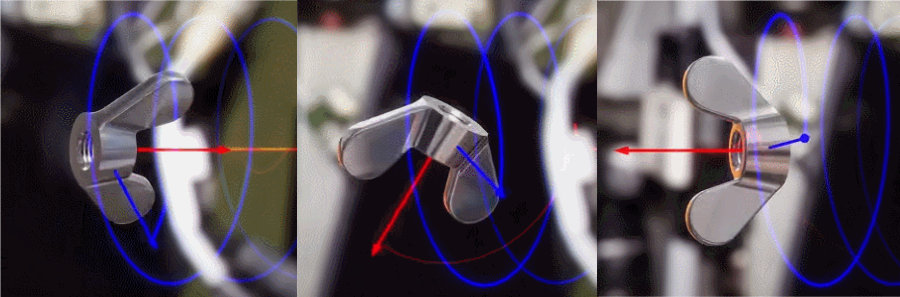
\includegraphics[width=0.9\textwidth]{dzhani.jpg}
\end{center}
   \caption{Satu gambaran tentang kesan Dzhanibekov \cite{28}.}
\label{fig:10}
\end{figure*}

Prinsip di sebalik perubahan pantas pada paksi putaran Bumi terletak pada fizik objek berputar. Contoh kanonik bagi ini ialah kesan Dzhanibekov, yang ditemui oleh angkasawan Rusia, Vladimir Dzhanibekov \cite{37}, dan digambarkan dalam Rajah \ref{fig:10}. Sesuatu objek yang tidak berputar dengan sempurna pada salah satu daripada tiga paksi inersia utamanya tidak akan mengekalkan paksi putaran yang tetap. Jika ia berputar hampir pada paksi utama kedua, ia akan melalui apa yang kelihatan sebagai perubahan mendadak dalam putaran. Walaupun ini bukanlah apa yang dipercayai berlaku semasa putaran pantas Bumi, intipatinya ialah tanpa adanya daya luar, hanya fizik putaran yang boleh menerangkan perubahan mendadak pada paksi putaran Bumi.

Untuk lebih tepat, Bumi hampir pasti tidak mengalami kesan Dzhanibekov yang mudah dan seragam. Jika ini berlaku, kita sepatutnya dapat mengesan perubahan beransur-ansur pada paksi putaran Bumi dari semasa ke semasa. Sebaliknya, kami percaya bahawa Bumi mengalami gangguan fizikal secara berkala dan tiba-tiba, yang menyebabkan "putaran luar" (kerak/mantel) dan "badan putaran dalam" (teras) Bumi terpisah. Tanpa input luar, hukum pemeliharaan momentum sudut menyatakan bahawa Bumi tidak boleh tiba-tiba menukar paksi putaran, jadi pemisahan antara badan putaran luar dan dalam adalah salah satu perkara yang jarang, selain daripada impak luar ke atas Bumi, yang boleh menyebabkan putaran mendadak dan tiba-tiba.

Proses khusus yang memacu gangguan dalaman di Bumi dipercayai adalah perubahan keadaan dalam struktur besi yang membentuk teras Bumi (Rajah \ref{fig:11}). Teras dalam terdiri daripada besi padat susunan heksagon (Fe) \cite{141}. Apabila hcp-Fe ini bertukar menjadi keadaan logam cecair, ia melepaskan tenaga kinetik, dan dialirkan ke teras luar. Perubahan fasa ini mengurangkan kebolehtelapan magnetik teras, melemahkan medan geomagnet, dan melepaskan haba, menghasilkan struktur LLVP (large low-velocity shear province) (Rajah \ref{fig:12}) \cite{38} dalam mantel, serta memanaskan permukaan Bumi melalui lautan abyssal. Kedua-dua pola ini telah banyak didokumentasikan dalam abad-abad kebelakangan ini dan akan dibincangkan kemudian dalam makalah ini.

\begin{figure*}[t]
\begin{center}
% \fbox{\rule{0pt}{2in} \rule{.9\linewidth}{0pt}}
\includegraphics[width=1\textwidth]{layers.jpg}
\end{center}
   \caption{Gambaran tentang proses dalaman Bumi yang membawa kepada flip ECDO \cite{129}.}
\label{fig:11}
\end{figure*}


\begin{figure}[t]
\begin{center}
% \fbox{\rule{0pt}{2in} \rule{0.9\linewidth}{0pt}}
   \includegraphics[width=1\linewidth]{llvp.jpg}
\end{center}
   \caption{Visual terperinci LLVP di bawah Afrika Selatan \cite{28}.}
\label{fig:12}
\label{fig:onecol}
\end{figure}


Proses yang sama di dalam Bumi ini, yang berlaku secara songsang, juga dipercayai mendorong peralihan kembali kepada keadaan putaran Bumi sekarang tidak lama selepas flip berlaku.

\section{Bukti untuk Flip Bumi yang Akan Datang}
There is strong reason to believe that we are on the brink of another Earth flip. A cataclysm has not occurred for several millennia, which is approximately the frequency with which these events seem to happen based on historical accounts and data. The strongest data supporting an impending flip comes from recent geomagnetic data, which indicates that the Earth's geomagnetic field has been weakening for approximately two thousand years. This weakening has been accelerating and has reached alarming rates in the last few decades.

Terdapat sebab yang kukuh untuk mempercayai bahawa kita berada di ambang satu lagi peralihan Bumi. Satu malapetaka tidak berlaku selama beberapa milenium, iaitu kira-kira kekerapan peristiwa-peristiwa ini nampaknya berlaku berdasarkan catatan sejarah dan data. Data terkuat yang menyokong kemungkinan peralihan yang akan berlaku datang daripada data geomagnetik terkini, yang menunjukkan bahawa medan geomagnetik Bumi telah melemah selama kira-kira dua ribu tahun. Pelemahan ini semakin mempercepatkan dan telah mencapai kadar yang membimbangkan dalam beberapa dekad terakhir.

Depicted in Figure \ref{fig:14} is the geomagnetic field of Earth in 1590 and 2025 \cite{125,126}. As shown in the figure, the field has weakened significantly.

Ditunjukkan dalam Rajah \ref{fig:14} ialah medan geomagnetik Bumi pada tahun 1590 dan 2025 \cite{125,126}. Seperti yang ditunjukkan dalam rajah tersebut, medan tersebut telah melemah dengan ketara.

Another metric for the weakening geomagnetic field is the position of the geomagnetic north pole (Figure \ref{fig:13}). Geomagnetic north has historically been located in the Canadian Arctic. However, it has been wandering slowly over the last several centuries, and accelerated significantly a few decades ago. It is now moving rapidly towards Russia at a rate of 55 kilometers per year \cite{124}.

Satu lagi metrik untuk kelemahan medan geomagnetik ialah kedudukan kutub utara geomagnetik (Rajah \ref{fig:13}). Utara geomagnetik secara sejarahnya terletak di Artik Kanada. Walau bagaimanapun, ia telah bergerak perlahan-lahan sejak beberapa abad yang lalu, dan telah mempercepatkan dengan ketara beberapa dekad yang lalu. Ia kini bergerak dengan pantas ke arah Rusia pada kadar 55 kilometer setahun \cite{124}.

\begin{figure*}[t]
\begin{center}
% \fbox{\rule{0pt}{2in} \rule{.9\linewidth}{0pt}}
\includegraphics[width=0.9\textwidth]{saa.jpg}
\end{center}
   \caption{Satu gambaran tentang pelemahan medan geomagnetik dari tahun 1590 hingga 2025. Dikira menggunakan model gufm1 dan IGRF-14 \cite{125,126}.}
\label{fig:14}
\end{figure*}

\begin{figure}[t]
\begin{center}
% \fbox{\rule{0pt}{2in} \rule{1\linewidth}{0pt}}
   \includegraphics[width=1\linewidth]{npw.jpg}
\end{center}

   \caption{Kedudukan kutub utara geomagnetik dari 1590 hingga 2025, digambarkan dalam kenaikan 5 tahun \cite{142}.}
\label{fig:13}
\label{fig:onecol}
\end{figure}

\begin{figure}[t]
\begin{center}
% \fbox{\rule{0pt}{2in} \rule{1\linewidth}{0pt}}
   \includegraphics[width=1\linewidth]{ocean-highlight.jpg}
\end{center}
   \caption{Kadar pemanasan lautan dalam (kedalaman $>$2000 m) dari 1991 hingga 2010, dibulatkan dengan warna merah \cite{132}.}
\label{fig:15}
\label{fig:onecol}
\end{figure}

Medan magnet bumi dipercayai dijana oleh dinamo dalaman - lajur bulat arus magma yang bergerak dalam teras luar bumi akibat putarannya \cite{123}. Pelemahan medan geomagnetik adalah satu simptom gangguan jauh di dalam bumi. Menurut teori ECDO, gangguan ini melepaskan haba dan akhirnya membawa kepada penyangkutan antara mantel dan teras, menyebabkan pembalikan bumi \cite{1}.

Terdapat banyak data yang membuktikan kehadiran proses eksotermik di dalam bumi. Kepanasan bumi didokumenkan oleh kenaikan suhu permukaan benua dan lautan \cite{127,128}, peningkatan paras CO2 atmosfera yang bergerak selari dengan plumbum haba bumi \cite{129,130}, dan penurunan keluasan ais laut global \cite{131}. Data menunjukkan bahawa peningkatan paras CO2 dan suhu bukanlah punca perubahan iklim "buatan manusia" sebaliknya, kesan hiliran daripada teras eksotermik \cite{129}.

Paling ketara, kajian kadar pemanasan di lautan dalam (kedalaman $>$2000 meter) menunjukkan bukan sahaja lautan dalam semakin panas, kadar pemanasan paling tinggi didapati di lapisan abisal (4000 - 6000 m). Pemanasan laut dalam ini mempunyai pusat di bawah 4000 meter \cite{132,129}, yang tidak mungkin berlaku sekiranya lautan dipanaskan dari atas oleh atmosfera. Data sebegini memberikan sokongan kukuh bahawa perubahan iklim dan geomagnetik baru-baru ini didorong oleh proses jauh di dalam bumi. Rajah \ref{fig:15} menunjukkan kadar pemanasan lautan dalam global dari 1991 hingga 2010 \cite{132}.
\section{Pemodelan Pembalikan Bumi yang Akan Datang}

\begin{figure}[b]
\begin{center}
% \fbox{\rule{0pt}{2in} \rule{1\linewidth}{0pt}}
   \includegraphics[width=1\linewidth]{saa-crop.jpeg}
\end{center}
   \caption{Satu pengiraan titik peralihan berdasarkan Anomali Atlantik Selatan menunjukkan tarikh 13 Mac 2059 \cite{125,126}.}
\label{fig:16}
\label{fig:onecol}
\end{figure}

Meramalkan masa pembalikan Bumi yang seterusnya adalah satu tugas yang kompleks. Pada masa ini, model terbaik yang kita ada untuk ini terletak pada medan geomagnetik Bumi - Anomali Atlantik Selatan (SAA). Kawasan ini di atas Atlantik Selatan mempunyai kekuatan medan geomagnetik yang paling lemah dan ditakrifkan sebagai kawasan dengan kekuatan medan di bawah 32,000 nanotesla \cite{135}, yang merupakan nilai medan paling lemah pada tahun 1590. Luas permukaan Anomali Atlantik Selatan meningkat daripada 1\% permukaan Bumi pada tahun 1590 kepada 21\% pada tahun 2025 \cite{136}.

Untuk mendapatkan anggaran bila Bumi boleh berbalik, saya memadankan data keluasan permukaan SAA kepada persamaan titik peralihan hukum kuasa, yang memodelkan satu sistem kompleks yang menghampiri satu peralihan kritikal, di mana sistem mengalami perubahan dramatik dan mendadak. Pengiraan saya memberikan tarikh peralihan ramalan pada 13 Mac 2059 (Rajah \ref{fig:16}). Ramalan ini akan menjadi semakin tepat apabila kita semakin hampir dengan peralihan tersebut \cite{136}.

Metrik lain seperti pergerakan paksi putaran, anomali cuaca, serta data seismik dan gunung berapi juga boleh membantu kita mendapatkan ramalan yang lebih baik tentang bila pembalikan Bumi seterusnya mungkin berlaku.

\section{Garis Masa Sejarah ECDO}
Walaupun menetapkan garis masa tepat bagi peristiwa ECDO lampau adalah sukar, nampaknya terdapat sekurang-kurangnya 2 peristiwa ECDO semasa Holosen. Perhatikan catatan yang diceritakan oleh Herodotus daripada pendeta Mesir bahawa, \textit{"daripada raja pertama hingga kepada pendeta Hephaistos yang memerintah terakhir, terdapat tiga ratus empat puluh satu generasi manusia... Dalam tempoh ini mereka berkata bahawa matahari telah bergerak empat kali dari tempat kebiasaan terbitnya, dan di mana ia kini terbenam, dari sana ia telah dua kali terbit, dan di tempat ia kini terbit ia telah dua kali terbenam"} \cite{32}. Plato, yang hidup pada abad kelima SM \cite{111}, menyatakan bahawa selepas banjir yang menenggelamkan Atlantis dalam satu hari dan satu malam 9,000 tahun sebelumnya, \textit{"sejak itu telah berlaku banyak banjir, dan sisa yang terselamat di kawasan pergunungan tidak mengetahui seni menulis, dan selama banyak generasi hanya berusaha untuk memperoleh keperluan hidup"} \cite{112}, yang menunjukkan terdapat lebih daripada dua terbalik sejak tamatnya Younger Dryas sekitar 9700 SM. Bukti fizikal yang dibincangkan sepanjang makalah ini dan dalam kajian saya \cite{2} memberikan bukti yang mencukupi untuk catatan Plato.

Tarikh calon terkini untuk terbalik ECDO adalah dalam tempoh 2300 hingga 1600 SM, di mana banyak catatan banjir malapetaka (Gun-Yu \cite{113,114,115}, Ogyges \cite{116,117}, Peru \cite{118,119}, Exodus \cite{120}), kemusnahan dan pengabaian tamadun (Mohenjo-Daro \cite{121}, Minoan Crete\cite{100,101}) dan anomali fizikal (peristiwa bond \cite{122}, peristiwa 4.2 ribu tahun \cite{90}) telah bertarikh. Tiada pertemuan bukti yang mencukupi yang lebih terkini daripada ini yang mencadangkan kejadian malapetaka besar.

\section{Kesimpulan}

Operasi NANOOK adalah satu usaha peninjauan Perang Dingin oleh Amerika Syarikat untuk memetakan Artik dan Pantai utara Soviet selepas Perang Dunia II \cite{137}. Semasa penyelidikan mereka, mereka mendapati bahawa kutub magnet berada 125 hingga 200 batu ke utara daripada kedudukan sepatutnya berdasarkan penemuan ekspedisi terdahulu. Oleh itu, \textit{"Dalam kalangan saintis kerajaan, timbul persoalan mengenai apa yang akan berlaku apabila kutub magnet dan kutub geografi bertepatan. Untuk menjawabnya, di bawah kawalan projek Dr. Paul A. Siple, Rand Corporation telah dikontrak bagi menjalankan kajian makmal menggunakan model bumi yang dibina daripada sfera sepusat – sfera dalaman mewakili teras besi cair bumi yang bercas elektromagnet dan paksinya menentukan kutub “magnet”; dan sfera luaran mewakili kerak bumi yang berputar di sekitar paksi “kutub geografi”. Melalui eksperimen berulang kali, didapati bahawa apabila kutub “magnet” menghampiri kutub “geografi”, kutub “magnet” pada satu ketika akan mempercepat kadar pertemuannya seolah-olah ditarik ke arah kutub “geografi” oleh daya memusat dan melompat untuk bertepatan; tetapi sebaliknya, kutub “magnet” akan dengan pantas “terbalik” sekitar kutub “geografi”, kemudian terputar menuju khatulistiwa seolah-olah oleh daya sentrifugal, dan akhirnya berada di kedudukan di mana kedua-dua paksi mempunyai perbezaan sekitar 89 darjah. Selepas “terbalik kutub” ini berlaku, paksi-paksi itu kemudian secara perlahan mula bersatu semula dalam tempoh yang panjang"} \cite{138,139}.

Kemudiannya, \textit{"Pada salah satu mesyuarat saintifik yang dihadiri oleh Mejar White di Pentagon pada awal 1948, para saintis membincangkan tentang kesesuaian memberi amaran kepada orang awam mengenai fenomena terbalik kutub yang bakal berlaku. Tiada seorang pun saintis bersetuju untuk menyembunyikan maklumat dari orang awam; tetapi, sebaliknya, mereka juga tidak dapat bersetuju bagaimana untuk menyebarkannya. Pengetahuan tentang fenomena ini, menurut sebilangan mereka, boleh dengan sendirinya memusnahkan moral masyarakat. Ketakutan mereka ternyata tidak berasas apabila, pada awal 1950-an, maklumat tentang fenomena terbalik itu disiarkan dalam ruangan akhbar dan artikel majalah, tetapi secara mengejutkan tidak mendapat maklum balas daripada masyarakat yang kelihatan terkejut, parokial atau tidak percaya"} \cite{138,139}.

Mengapa kita tidak memberikan perhatian terhadap perkara ini? Terdapat sebab yang kukuh untuk mempercayai bahawa Bumi pernah terbalik sebelum ini. Makalah ini, bersama dengan bahagian kedua makalah, memberikan ringkasan padat tentang pelbagai bukti dari banyak bidang yang menunjukkan perkara ini, seperti kisah banjir di seluruh dunia, fosil garam dan fosil marin yang merangkumi benua-benua, tempat perlindungan bawah tanah purba, sisa haiwan, dan landskap geologi malapetaka. Manusia dikatakan berusia ratusan ribu tahun, namun sejarah moden hanya bermula beberapa ribu tahun yang lalu. Tidakkah mungkin setiap beberapa ketika, Bumi terbalik, benua-benua dibersihkan, dan kita terpaksa kembali semula ke tahap permulaan – Zaman Batu – dan rekod sejarah purba kita hanya tinggal beberapa kisah malapetaka? Jika begitu, maka mengelakkan perkara ini daripada berulang mungkin merupakan salah satu tugas terpenting manusia.

Akhir kata, saya tinggalkan anda dengan catatan yang diceritakan dalam Timaeus, tulisan Plato, tentang perbualan antara Solon, seorang negarawan Athens, dan pendeta Mesir \cite{140}: \textit{"Dan pada satu ketika, apabila [Solon] ingin membawa mereka berbicara mengenai sejarah kuno, beliau cuba menceritakan kepada mereka tradisi kita yang paling kuno, mengenai Phoroneus, yang dikatakan sebagai manusia pertama, dan Niobe; dan beliau terus menceritakan legenda tentang Deucalion dan Pyrrha selepas Banjir, dan bagaimana mereka terselamat, dan memberikan silsilah keturunan mereka; dan dengan menghitung bilangan tahun yang diambil oleh peristiwa yang disebutkan, beliau cuba mengira tempoh masa. Lalu salah seorang pendeta, seorang yang sangat tua, berkata, “Wahai Solon, Solon, kamu orang Yunani sentiasa muda: tiada satu pun perkara seperti orang Yunani tua.” Dan setelah mendengar ini beliau bertanya, “Apa maksud kata-kata ini?” Dan pendeta itu menjawab, “Kamu semua muda dalam jiwa. Ini kerana kamu tidak memiliki satu kepercayaan pun yang kuno dan diwarisi daripada tradisi lama, apatah lagi satu ilmu yang sudah lama. Dan inilah sebabnya: Terdapat dan akan ada banyak kemusnahan pelbagai jenis ke atas manusia, yang paling besar oleh api dan air, dan yang lebih kecil oleh pelbagai cara yang tak terhitung. Sesungguhnya kisah yang diceritakan di negerimu dan juga di negara kami, tentang bagaimana suatu ketika dahulu Phaethon, anak Helios, menunggang kereta kuda ayahnya, dan, kerana dia tidak dapat mengendalikannya seperti ayahnya, membakar segala yang ada di bumi dan dirinya sendiri terbunuh oleh panahan petir — kisah itu, seperti diceritakan, kelihatan seperti legenda, tetapi kebenarannya terletak pada peristiwa perubahan kedudukan jasad-jasad di langit yang bergerak mengelilingi bumi, dan kemusnahan benda-benda di bumi oleh api yang dahsyat, yang berlaku dalam selang masa yang panjang. Pada masa itu, semua yang tinggal di gunung-gunung dan tempat tinggi serta kering mengalami kemusnahan lebih daripada mereka yang tinggal berdekatan sungai atau laut; dan dalam kes kami, Sungai Nil, yang menjadi Penyelamat kami dalam pelbagai cara, menyelamatkan kami juga pada masa itu dengan naik tinggi. Dan apabila, sebaliknya, Para Dewa membersihkan bumi dengan banjir air, semua penggembala dan penjaga ternakan yang berada di gunung diselamatkan, tetapi mereka yang di bandar-bandar di negaramu dihanyutkan ke laut oleh arus sungai; manakala di negara kami air tidak pernah dan tidak akan turun membanjiri ladang kami dari atas, sebaliknya ia sentiasa cenderung untuk timbul dari bawah. Oleh itu, kerana sebab-sebab ini, apa yang dipelihara di sini dianggap paling kuno; kebenarannya, di mana-mana tempat yang tiada panas atau sejuk yang melampau untuk menghalangnya, sentiasa ada manusia, kadang ramai, kadang sedikit. Dan jika berlaku sesuatu peristiwa yang mulia atau agung atau dengan apa cara sekalipun menonjol, sama ada di negaramu, kami atau di tempat lain yang kami ketahui, semua peristiwa seperti itu direkodkan sejak dahulu kala dan dipelihara di sini di kuil-kuil kami; manakala bangsa kamu dan yang lain-lain sentiasa baru, setiap kali, dengan huruf dan seni yang diperlukan negeri beradab, dan, selepas tempoh lazim beberapa tahun, seperti wabak, banjir dari langit melanda rakyatmu, tidak meninggalkan sesiapa kecuali yang buta huruf dan tidak berbudaya, sehingga kamu menjadi muda semula, tanpa pengetahuan tentang segala yang berlaku suatu masa dahulu di sini atau di negaramu sendiri. Sudah tentu silsilah yang kamu ceritakan tadi, Solon, mengenai rakyat negaramu, tidak lebih daripada kisah kanak-kanak; kerana, pertama, kamu hanya mengingati satu banjir besar, walaupun banyak telah berlaku sebelumnya; dan seterusnya, kamu tidak tahu bahawa bangsa paling mulia dan sempurna dalam kalangan manusia lahir di tempat kamu sekarang tinggal, dan dari merekalah kamu dan seluruh kota kamu wujud, daripada benih kecil yang masih berbaki; tetapi ini terlepas pandang kerana selama banyak generasi yang terselamat mati tanpa mampu menzahirkan diri secara bertulis. Sesungguhnya pada satu masa, Solon, sebelum kemusnahan besar oleh air, negeri Athens yang ada kini adalah yang paling berani dalam peperangan dan teratur dalam semua aspek lain. Dikatakan bahawa ia memiliki hasil seni yang paling hebat dan sistem pemerintahan paling mulia daripada mana-mana bangsa di bawah langit yang pernah kami dengar.”}

Pendeta-pendeta yang sama inilah, semestinya, turut menceritakan kepada Solon mengenai tamadun purba Atlantis: \textit{"Kerana semua yang ada di sini, terletak di dalam muara yang kami sebutkan, jelas merupakan pelabuhan dengan pintu masuk yang sempit; tetapi yang di sana adalah lautan sebenar, dan tanah yang mengelilinginya boleh dipanggil, dengan tepat dan benar, sebuah benua. Kini di pulau Atlantis terdapat satu persekutuan raja-raja, berkuasa besar dan menakjubkan, yang memerintah seluruh pulau, dan juga banyak pulau lain serta sebahagian benua; lebih-lebih lagi, tanah di dalam Selat mereka memerintah Libya hingga ke Mesir, dan Eropah hingga ke Tyrrhenia. Maka, dengan kekuatan besar itu, mereka pernah cuba menakluk sekaligus negara kamu dan negara kami serta seluruh kawasan dalam Selat. Dan pada waktu itulah, Solon, keberanian bangsa kamu nyata menonjol di hadapan seluruh dunia. Ia unggul dalam keberanian dan kesenian peperangan, dan bertindak sebahagiannya sebagai ketua Yunani, dan sebahagiannya berdiri sendiri apabila ditinggalkan yang lain; setelah menghadapi bahaya paling besar, ia menewaskan penceroboh dan mendirikan trofi; daripadanya, ia menyelamatkan mereka yang belum diperhambakan, dan semua yang lain yang hidup dalam jajaran Heracles dibebaskan tanpa sekatan. Tetapi kemudian berlaku gempa bumi dan banjir besar, dan satu hari dan malam yang amat dahsyat menimpa mereka, apabila seluruh tentera kamu ditelan bumi, dan pulau Atlantis juga ditelan laut dan lenyap"}.

\section{Penghargaan}

Terima kasih kepada Ethical Skeptic, penulis asal tesis ECDO, kerana menyiapkan tesisnya yang penuh wawasan dan revolusioner dan berkongsi dengan dunia. Tesis tiga bahagiannya \cite{1} kekal menjadi karya utama untuk teori Exothermic Core-Mantle Decoupling Dzhanibekov Oscillation (ECDO), dan mengandungi maklumat yang jauh lebih banyak tentang topik ini berbanding yang sempat saya ulas di sini.
Terima kasih kepada Ankit, yang telah memproses data kompilasi malapetaka dalam Jadual 1.

Dan sudah tentu, terima kasih kepada para gergasi yang menjadi tempat kita berpijak; mereka yang telah menjalankan semua penyelidikan dan siasatan yang memungkinkan kerja ini dan berusaha membawa cahaya kepada kemanusiaan.

\clearpage
\twocolumn

\section{Imej Tambahan}


\begin{figure}[H]
\begin{center}
% \fbox{\rule{0pt}{2in} \rule{1\linewidth}{0pt}}
   \includegraphics[width=1\linewidth]{wave.jpg}
\end{center}
   \caption{Pandangan dekat pada hakisan gelombang parabola, terpotong di Piramid Khafre \cite{27}.}
\label{fig:19}
\label{fig:onecol}
\end{figure}
\begin{figure}[H]
\begin{center}
% \fbox{\rule{0pt}{2in} \rule{1\linewidth}{0pt}}
   \includegraphics[width=1\linewidth]{star-stone.jpg}
\end{center}
   \caption{Peta bintang yang diukir pada batu di salah satu saluran piramid Khufu \cite{28}.}
\label{fig:20}
\label{fig:onecol}
\end{figure}

\begin{figure*}[t]
\begin{center}
% \fbox{\rule{0pt}{2in} \rule{.9\linewidth}{0pt}}
\includegraphics[width=1\textwidth]{deepsea.jpg}
\end{center}
   \caption{Visual anomali pemanasan lautan dalam dan jurang berbanding dengan lengkung pemanasan atmosfera laut yang normal. Jumlah keseluruhan anomali pemanasan diambil daripada NOAA \cite{147}, taburan pemanasan dalam dan jurang daripada kajian Desbruyeres \cite{132}, dan pemprosesan serta visualisasi data oleh Ethical Skeptic \cite{129}.}
\label{fig:21}
\end{figure*}
\begin{figure*}[t]
\begin{center}
% \fbox{\rule{0pt}{2in} \rule{.9\linewidth}{0pt}}
\includegraphics[width=1\textwidth]{sealevel.jpeg}
\end{center}
   \caption{Paras laut menunjukkan peningkatan varians sebanyak 20\% dalam tempoh 75 tahun di 63 stesen, menunjukkan peningkatan dalam kelajuan arus. Lonjakan dalam varians paras laut berlaku serentak dengan denyut haba lautan, menunjukkan kedua-duanya mungkin disebabkan oleh pemanasan dari jauh di bawah lautan Bumi \cite{2,129}.}
\label{fig:22}
\end{figure*}

\begin{figure*}[t]
\begin{center}
% \fbox{\rule{0pt}{2in} \rule{.9\linewidth}{0pt}}
\includegraphics[width=1\textwidth]{co2.jpg}
\end{center}
   \caption{PPM CO2 atmosfera telah meningkat secara konsisten dalam tempoh 45 tahun yang lepas, berkemungkinan disebabkan oleh kenaikan suhu lautan. Sumber: NOAA \cite{148,129}.}
\label{fig:23}
\end{figure*}

\begin{figure*}[t]
\begin{center}
% \fbox{\rule{0pt}{2in} \rule{.9\linewidth}{0pt}}
\includegraphics[width=1\textwidth]{ice.jpg}
\end{center}
   \caption{Luas ais laut global telah menyusut sepanjang 45 tahun yang lalu, akibat pemanasan Bumi. Sumber: ADS \cite{149}.}
\label{fig:24}
\end{figure*}

\clearpage
\twocolumn

{\small
\renewcommand{\refname}{Rujukan}
\bibliographystyle{ieee}
\bibliography{egbib}
}

\end{document}